\newpage
\hypertarget{remCard tex}{}
\subsection{Implementing removeCard}
\texHeader

\begin{itemize}

\item[$\blacktriangleright$] Go to the \texttt{removeCard} signature in the \texttt{Partition.eclass} file. Fill the method with a single pattern call,
\texttt{[deleteSingleCard]} and a return statement (Fig~\ref{fig:remCardDec}).

\begin{figure}[htp]
\begin{center}
  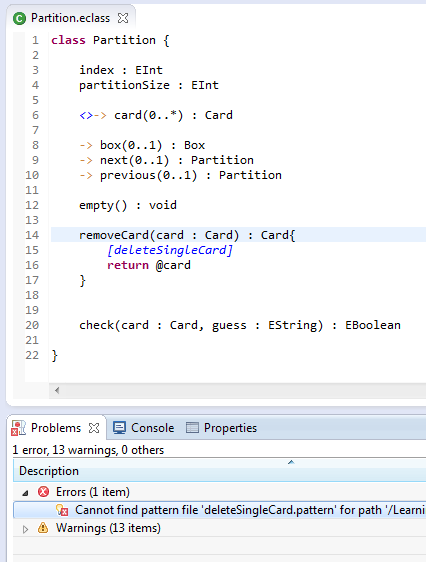
\includegraphics[width=0.5\textwidth]{eclipse_removeCardDeclaration}
  \caption{Control flow for \texttt{removeCard}}
  \label{fig:remCardDec}
\end{center}
\end{figure}

\item[$\blacktriangleright$] To lightly touch on MOSL syntax, the `@' operator refers to a \emph{bound} variable. In this method, \texttt{card} is bound since
it is the passed-in variable.

\item[$\blacktriangleright$] As soon as you save the file, an error should immediately appear. In the ``Problems'' tab below the editor, the message states that
the builder cannot find the specified pattern file. Well, that makes sense - you haven't made it yet! Click this message and press \texttt{Control + 1} to
invoke a ``Quick Fix'' dialouge (Fig~\ref{fig:quixFix})

\begin{figure}[htp]
\begin{center}
  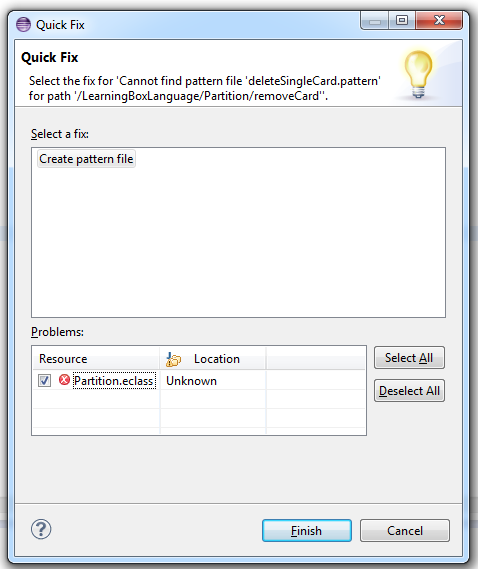
\includegraphics[width=0.6\textwidth]{eclipse_patternQuickFix}
  \caption{A quick solution to a pattern error}
  \label{fig:quixFix}
\end{center}
\end{figure}

\item[$\blacktriangleright$] It offers to create a pattern file for you. Given that's exactly what you'd like to do, select the option and press
\texttt{Finish}.

\item[$\blacktriangleright$] The new file will open in the editor, and a new directory structure will appear under ``\_patterns'' (Fig.~\ref{fig:pattStruct}). SDMs are
placed in SDM containers, named according to the method they implement. In this case, \texttt{deleteSingleCard.pattern} is invoked by the method \texttt{removeCard},
which itself is found in the \texttt{Partition} class. \texttt{Partition} will eventually contain folders for each method that implements a pattern.

\begin{figure}[htp]
\begin{center}
  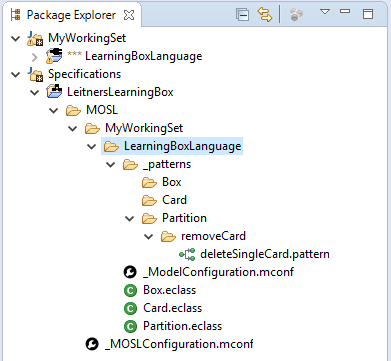
\includegraphics[width=0.9\textwidth]{eclipse_patternStructure}
  \caption{Directory structure for a pattern}
  \label{fig:pattStruct}
\end{center}
\end{figure}

% don't forget to discuss syntax!
\item[$\blacktriangleright$] The content of any pattern file is simply a list of tasks and rules. You create a series of \emph{Object Variables}, and then,
within those declarations, state operations such as `delete this reference'.\footnote{Hint, hint!} Remember - the focus here is not on how, but on what.

\item[$\blacktriangleright$] Create two rules, \texttt{@this:Partition\{ \}} and~\texttt{@card:Card\{ \}}~(Fig.~\ref{fig:remCardObjVar}). Just like parameter
values, \texttt{this} variables are always bounded.

\item[$\blacktriangleright$] eMoflon offers type completion to assist you when declaring items in your metamodel. Simply press \texttt{control + space} before
typing to see your options.

\begin{figure}[htp]
\begin{center}
  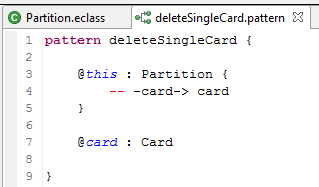
\includegraphics[width=0.6\textwidth]{eclipse_remCardObjVars}
  \caption{Object variables for \texttt{removeCard}}
  \label{fig:remCardObjVar}
\end{center}
\end{figure}

\clearpage

\item[$\blacktriangleright$] Add `\texttt{-- -> card:card}' to \texttt{@this} to destroy the \texttt{card} reference targeting the \texttt{card} object. The key
spaces of your workspace should now resemble Fig.~\ref{fig:deleteReference}.

\begin{figure}[htp]
\begin{center}
  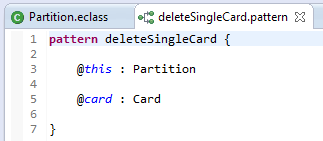
\includegraphics[width=0.6\textwidth]{eclipse_thisObjVar}
  \caption{Destroy the link between a card and its partition {\bf add declaration}}
  \label{fig:deleteReference}
\end{center}
\end{figure}

\item[$\blacktriangleright$] If you ever need to quickly remind yourself of specific navigation names or attributes, press \texttt{alt} and the left arrow to
jump back to your eclass. Conversely, to quickly open or jump to a pattern, Hover over the pattern name while holding \texttt{control} until it's underlined, then click!

\item[$\blacktriangleright$] Remember that links between classes are defined via \emph{Bidrectional EReferences},\footnote{technically two
\emph{unidirectional EReferences}} linked together as opposites in ``LearningBoxLanguage/\_con\-straints.mconf.'' This means we can leave the second rule empty,
as declaring \texttt{-- -> cardContainer:Card} would be redundant.

\item[$\blacktriangleright$] Build your project and navigate to ``MyWorkingSet/LearningBoxLanguage/gen." Open ``Partition.impl'' and scroll down to the
\texttt{RemoveCard} declaration. If everything compiled without errors, you should be able to see some generated code (Fig.~\ref{fig:remCardImpl}).

\begin{figure}[htp]
\begin{center}
  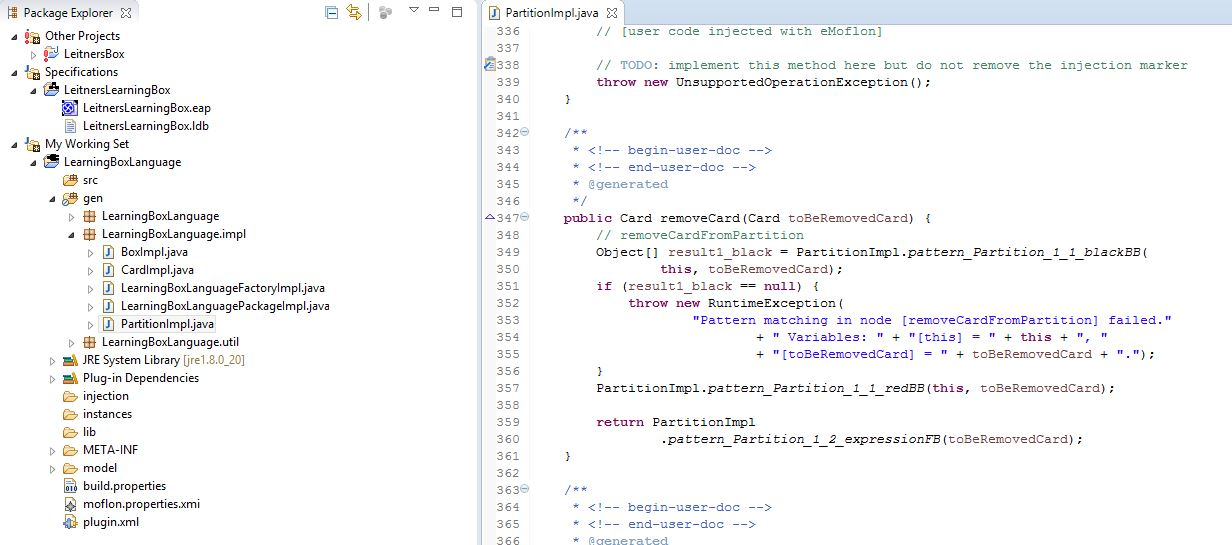
\includegraphics[width=\textwidth]{eclipse_remCardImpl}
  \caption{Generated implementation code}
  \label{fig:remCardImpl}
\end{center}
\end{figure}

\item[$\blacktriangleright$] Given that we were able to actually remove a card from our Box using injections, lets test \emph{this} implementation using our GUI
(Fig.~\ref{fig:GUITest}).\footnote{ If you haven't downloaded or used the GUI before, review Part II, section 7} If it doesn't work for you, inspect your
pattern class and confirm it matches Fig.~\ref{fig:deleteReference}.

\begin{figure}[htp]
\begin{center}
  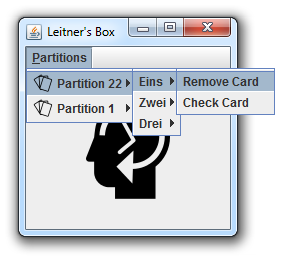
\includegraphics[width=0.5\textwidth]{eclipse_remCardGUITest}
  \caption{Testing implementation with the GUI}
  \label{fig:GUITest}
\end{center}
\end{figure}

\item[$\blacktriangleright$] Fantastic work! You have now implemented a simple reference manipulation via patterns. As you could see, SDM is effective for
implementing large functions that could potentially take a \emph{very} long time. To see how this same method is crafted in the visual syntax, check out
Fig.~\ref{fig:sdm_complete_control_flow} from the previous section.

% \fancyfoot[R]{ $\triangleright$ \hyperlink{sec:checkCard}{Next} }

\end{itemize}
